\hypertarget{locator_8cpp}{}\section{app/locator.cpp File Reference}
\label{locator_8cpp}\index{app/locator.\+cpp@{app/locator.\+cpp}}


End result of class is to return the position of the object desired. Class will receive dimensions and starting pixel position of a bounding box, and from there determine the world coordinate position depending on the camera. Here we assume the intrinsic and extrinsic parameters of the camera.  


{\ttfamily \#include $<$iostream$>$}\\*
{\ttfamily \#include $<$opencv2/opencv.\+hpp$>$}\\*
{\ttfamily \#include $<$string$>$}\\*
{\ttfamily \#include $<$vector$>$}\\*
{\ttfamily \#include \char`\"{}locator.\+hpp\char`\"{}}\\*
Include dependency graph for locator.\+cpp\+:
\nopagebreak
\begin{figure}[H]
\begin{center}
\leavevmode
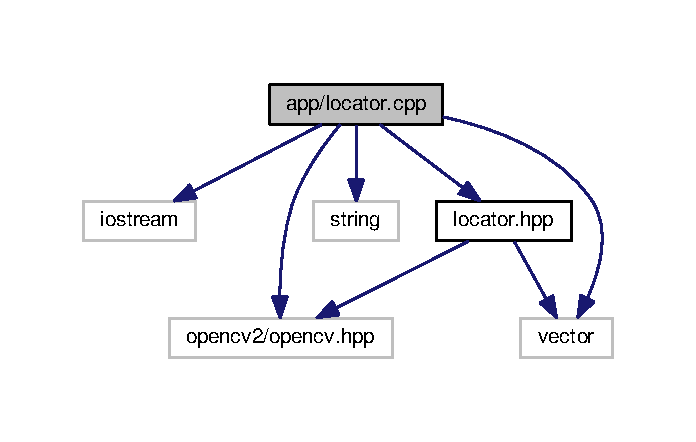
\includegraphics[width=334pt]{locator_8cpp__incl}
\end{center}
\end{figure}


\subsection{Detailed Description}
End result of class is to return the position of the object desired. Class will receive dimensions and starting pixel position of a bounding box, and from there determine the world coordinate position depending on the camera. Here we assume the intrinsic and extrinsic parameters of the camera. 

\begin{DoxyAuthor}{Author}
Pablo Sanhueza 

Andre Gomes 

Ryan Cunningham
\end{DoxyAuthor}
\begin{DoxyCopyright}{Copyright}
2019 Pablo Sanhueza, Andre Gomes, Ryan Cunningham 
\end{DoxyCopyright}
